\documentclass{ximera}

 

\usepackage{epsfig}

\graphicspath{
  {./}
  {figures/}
}

\usepackage{morewrites}
\makeatletter
\newcommand\subfile[1]{%
\renewcommand{\input}[1]{}%
\begingroup\skip@preamble\otherinput{#1}\endgroup\par\vspace{\topsep}
\let\input\otherinput}
\makeatother

\newcommand{\includeexercises}{\directlua{dofile("/home/jim/linearAlgebra/laode/exercises.lua")}}

%\newcounter{ccounter}
%\setcounter{ccounter}{1}
%\newcommand{\Chapter}[1]{\setcounter{chapter}{\arabic{ccounter}}\chapter{#1}\addtocounter{ccounter}{1}}

%\newcommand{\section}[1]{\section{#1}\setcounter{thm}{0}\setcounter{equation}{0}}

%\renewcommand{\theequation}{\arabic{chapter}.\arabic{section}.\arabic{equation}}
%\renewcommand{\thefigure}{\arabic{chapter}.\arabic{figure}}
%\renewcommand{\thetable}{\arabic{chapter}.\arabic{table}}

%\newcommand{\Sec}[2]{\section{#1}\markright{\arabic{ccounter}.\arabic{section}.#2}\setcounter{equation}{0}\setcounter{thm}{0}\setcounter{figure}{0}}

\newcommand{\Sec}[2]{\section{#1}}

\setcounter{secnumdepth}{2}
%\setcounter{secnumdepth}{1} 

%\newcounter{THM}
%\renewcommand{\theTHM}{\arabic{chapter}.\arabic{section}}

\newcommand{\trademark}{{R\!\!\!\!\!\bigcirc}}
%\newtheorem{exercise}{}

\newcommand{\dfield}{{\sf dfield9}}
\newcommand{\pplane}{{\sf pplane9}}

\newcommand{\EXER}{\section*{Exercises}}%\vspace*{0.2in}\hrule\small\setcounter{exercise}{0}}
\newcommand{\CEXER}{}%\vspace{0.08in}\begin{center}Computer Exercises\end{center}}
\newcommand{\TEXER}{} %\vspace{0.08in}\begin{center}Hand Exercises\end{center}}
\newcommand{\AEXER}{} %\vspace{0.08in}\begin{center}Hand Exercises\end{center}}

% BADBAD: \newcommand{\Bbb}{\bf}

\newcommand{\R}{\mbox{$\Bbb{R}$}}
\newcommand{\C}{\mbox{$\Bbb{C}$}}
\newcommand{\Z}{\mbox{$\Bbb{Z}$}}
\newcommand{\N}{\mbox{$\Bbb{N}$}}
\newcommand{\D}{\mbox{{\bf D}}}
\usepackage{amssymb}
%\newcommand{\qed}{\hfill\mbox{\raggedright$\square$} \vspace{1ex}}
%\newcommand{\proof}{\noindent {\bf Proof:} \hspace{0.1in}}

\newcommand{\setmin}{\;\mbox{--}\;}
\newcommand{\Matlab}{{M\small{AT\-LAB}} }
\newcommand{\Matlabp}{{M\small{AT\-LAB}}}
\newcommand{\computer}{\Matlab Instructions}
\newcommand{\half}{\mbox{$\frac{1}{2}$}}
\newcommand{\compose}{\raisebox{.15ex}{\mbox{{\scriptsize$\circ$}}}}
\newcommand{\AND}{\quad\mbox{and}\quad}
\newcommand{\vect}[2]{\left(\begin{array}{c} #1_1 \\ \vdots \\
 #1_{#2}\end{array}\right)}
\newcommand{\mattwo}[4]{\left(\begin{array}{rr} #1 & #2\\ #3
&#4\end{array}\right)}
\newcommand{\mattwoc}[4]{\left(\begin{array}{cc} #1 & #2\\ #3
&#4\end{array}\right)}
\newcommand{\vectwo}[2]{\left(\begin{array}{r} #1 \\ #2\end{array}\right)}
\newcommand{\vectwoc}[2]{\left(\begin{array}{c} #1 \\ #2\end{array}\right)}

\newcommand{\ignore}[1]{}


\newcommand{\inv}{^{-1}}
\newcommand{\CC}{{\cal C}}
\newcommand{\CCone}{\CC^1}
\newcommand{\Span}{{\rm span}}
\newcommand{\rank}{{\rm rank}}
\newcommand{\trace}{{\rm tr}}
\newcommand{\RE}{{\rm Re}}
\newcommand{\IM}{{\rm Im}}
\newcommand{\nulls}{{\rm null\;space}}

\newcommand{\dps}{\displaystyle}
\newcommand{\arraystart}{\renewcommand{\arraystretch}{1.8}}
\newcommand{\arrayfinish}{\renewcommand{\arraystretch}{1.2}}
\newcommand{\Start}[1]{\vspace{0.08in}\noindent {\bf Section~\ref{#1}}}
\newcommand{\exer}[1]{\noindent {\bf \ref{#1}}}
\newcommand{\ans}{}
\newcommand{\matthree}[9]{\left(\begin{array}{rrr} #1 & #2 & #3 \\ #4 & #5 & #6
\\ #7 & #8 & #9\end{array}\right)}
\newcommand{\cvectwo}[2]{\left(\begin{array}{c} #1 \\ #2\end{array}\right)}
\newcommand{\cmatthree}[9]{\left(\begin{array}{ccc} #1 & #2 & #3 \\ #4 & #5 &
#6 \\ #7 & #8 & #9\end{array}\right)}
\newcommand{\vecthree}[3]{\left(\begin{array}{r} #1 \\ #2 \\
#3\end{array}\right)}
\newcommand{\cvecthree}[3]{\left(\begin{array}{c} #1 \\ #2 \\
#3\end{array}\right)}
\newcommand{\cmattwo}[4]{\left(\begin{array}{cc} #1 & #2\\ #3
&#4\end{array}\right)}

\newcommand{\Matrix}[1]{\ensuremath{\left(\begin{array}{rrrrrrrrrrrrrrrrrr} #1 \end{array}\right)}}

\newcommand{\Matrixc}[1]{\ensuremath{\left(\begin{array}{cccccccccccc} #1 \end{array}\right)}}



\renewcommand{\labelenumi}{\theenumi)}
\newenvironment{enumeratea}%
{\begingroup
 \renewcommand{\theenumi}{\alph{enumi}}
 \renewcommand{\labelenumi}{(\theenumi)}
 \begin{enumerate}}
 {\end{enumerate}\endgroup}



\newcounter{help}
\renewcommand{\thehelp}{\thesection.\arabic{equation}}

%\newenvironment{equation*}%
%{\renewcommand\endequation{\eqno (\theequation)* $$}%
%   \begin{equation}}%
%   {\end{equation}\renewcommand\endequation{\eqno \@eqnnum
%$$\global\@ignoretrue}}

%\input{psfig.tex}

\author{Martin Golubitsky and Michael Dellnitz}

%\newenvironment{matlabEquation}%
%{\renewcommand\endequation{\eqno (\theequation*) $$}%
%   \begin{equation}}%
%   {\end{equation}\renewcommand\endequation{\eqno \@eqnnum
% $$\global\@ignoretrue}}

\newcommand{\soln}{\textbf{Solution:} }
\newcommand{\exercap}[1]{\centerline{Figure~\ref{#1}}}
\newcommand{\exercaptwo}[1]{\centerline{Figure~\ref{#1}a\hspace{2.1in}
Figure~\ref{#1}b}}
\newcommand{\exercapthree}[1]{\centerline{Figure~\ref{#1}a\hspace{1.2in}
Figure~\ref{#1}b\hspace{1.2in}Figure~\ref{#1}c}}
\newcommand{\para}{\hspace{0.4in}}

\renewenvironment{solution}{\suppress}{\endsuppress}

\ifxake
\newenvironment{matlabEquation}{\begin{equation}}{\end{equation}}
\else
\newenvironment{matlabEquation}%
{\let\oldtheequation\theequation\renewcommand{\theequation}{\oldtheequation*}\begin{equation}}%
  {\end{equation}\let\theequation\oldtheequation}
\fi

\makeatother


\title{Graphing Solutions to Differential Equations}

\begin{document}
\begin{abstract}
\end{abstract}
\maketitle


\label{S:3.2}

Solutions to differential equations can be graphed in several
different ways, each giving different insight into the structure
of the solutions.  We begin by asking what object is to be
graphed.  Do we first solve the differential equation and then
graph the solution, or do we let the computer find the solution
numerically and then graph the result?  The first method assumes
that we can find a formula for the solution (such as
$x(t)=x_0e^{\lambda t}$).  A solution to a differential equation
for which we have an explicit formula is called a {\em closed
form\/} solution\index{closed form solution}.  Using \Matlab we
can graph closed form solutions, as we showed in
Figure~\ref{graph_labelfig}. The second method of graphing
solutions requires having a numerical method that can {\em
numerically integrate\/} the differential equation to any
desired degree of accuracy.

In fact, there are rather few differential equations that can be
solved in closed form (though the linear systems that we
describe in this chapter are ones that can be solved in closed
form).  Without formulas, the first method is impossible.  There
are, however, several efficient algorithms for the numerical
solution of (systems of) ordinary differential equations and
these methods have been preprogrammed in \Matlabp.  In our
discussions, we treat \Matlab as a {\em black box\/} numerical
integration solver of ordinary differential equations.

\subsection*{A Single First Order Ordinary Differential Equation}

We begin our discussion of the numerical integration of
differential equations with the single first order \index{first
order}\index{differential equation!first order} differential equation
of the form:
\begin{equation} \label{nonaut}
\frac{dx}{dt}(t) = f(t,x(t)).
\end{equation}
The equation is {\em first order\/} since only the first
derivative of the function $x(t)$ appears in the equation. If
the second derivative appeared in the equation, then the equation
would be a second order equation.

\subsubsection*{Independent ($t$) and Dependent ($x$) Variables}

Sometimes this equation is also written in the form
\begin{equation}  \label{nonaut2}
	\frac{dx}{dt} = f(t,x)
\end{equation}
and in this form both $t$ and $x$ appear as variables.  But $x$
is a function $x(t)$ depending on $t$, and therefore the
variable $t$ is called the {\em independent\/}
\index{independent variable} variable, while the variable $x$ is
called the {\em dependent\/} \index{dependent variable} variable.

\subsubsection*{Autonomous versus Nonautonomous}

When the right hand side $f$ does not depend explicitly on the
independent time variable $t$, then the equation is called {\em
autonomous\/}\index{autonomous}\index{differential equation!autonomous}.
More explicitly, in
\Ref{nonaut2}, the differential equation is autonomous when
$f(t,x)=g(x)$.  Equation \Ref{lin1} is an example of an
autonomous differential equation since $f(t,x)=\lambda x$.

When $f$ depends explicitly on the independent time variable $t$,
the differential equation is called {\em nonautonomous\/}.
\index{nonautonomous}\index{differential equation!nonautonomous}
Suppose in our example of interest rates  in Section~\ref{S:growthmodels}
we had assumed that the interest rate $r$ changes in time.  In
such a case we would write $r=r(t)$ and the differential equation modeling 
how the principal $P(t)$ changes in time would be written as
\begin{equation}  \label{E:varinterest}
\frac{dP}{dt} = r(t)P.
\end{equation}
This equation is an example of a nonautonomous differential equation 
since $f(t,P) = r(t)P$.   For instance, suppose that at time $t=0$ the
principal in our account is $P_0$, and the interest rate is $5.5\%$.  
Now suppose the bank changes the interest rate after six months to $4.5\%$. 
Then $P(t)$ is a solution to \Ref{E:varinterest}, where
\[
  r(t) = \left\{\begin{array}{l}
     0.055\quad\mbox{for $0\le t < 0.5$, and}\\
     0.045\quad\mbox{for $0.5\le t$,}
  \end{array}\right.
\]
and $P(0)=P_0$.

Another example of a nonautonomous differential equation is given by
\begin{equation}  \label{dfeq}
\frac{dx}{dt} = x^2-t.
\end{equation}


\subsection*{Time Series and Phase Space Plots}

There are two different methods for visualizing the result of
numerical integration of differential equations of the form
\Ref{nonaut}: time series plots and phase space plots.  These
two methods are based on interpreting the derivative $dx/dt$
alternatively as either the slope of a tangent line or as the
velocity of a particle.

A {\em time series\/} \index{time series} plot for a solution to
\Ref{nonaut} is found by plotting $x$ versus $t$ as we did for
the closed form solution in Figure~\ref{graph_labelfig}.  However,
when graphing time series of solutions we do not need to find closed
form solutions.  To understand how this is done, we briefly discuss
what equation \Ref{nonaut} is actually saying about a solution
$x(t)$.  This equation states that the slope of the tangent line
to the graph of the function $x(t)$ at time t ($dx/dt$) is known
and equals $f(t,x(t))$.  Thus we can use the right hand side of
\Ref{nonaut} to draw the tangent lines to $x(t)$ at each point
in the $tx$-plane.  This leads to the notion of a line field.
The rough idea behind the numerical integration scheme is to fit
a curve $(t,x(t))$ into the $tx$-plane in such a way that the
tangent lines to the curve match the tangent lines specified by
the slope $f$.

A {\em phase space\/} \index{phase!space} plot is based on
the {\em other\/} interpretation of a derivative as a rate of
change --- a velocity.  We let $x(t)$ denote the position of a
particle on the real line at time $t$.  The function $f(t,x)$
denotes the velocity of that particle when the particle is at
position $x$ at time $t$.  Thus, to view the phase space plot,
we need to see the particle moving along the real line; that is,
we need to see how $x(t)$ changes in $t$.  Later, we will use
\Matlab graphics to actually visualize the particle movement.

Thus time series are graphs of functions in the $tx$-plane while
phase space plots are graphs on the real line $x$.  We discuss
time series plots in this section and phase line plots in the
next.


\subsection*{Line Fields}

We begin our discussion of line fields \index{line field} (or
synonymously direction fields) \index{direction field} by
focusing on the information about solutions that can directly
be extracted from the equation itself.  To illustrate this we
consider the differential equation \Ref{dfeq}.

As mentioned, the differential equation $\dot{x}=x^2-t$ reflects the fact 
that the value of the derivative of a solution $x(t)$ at time $t$ is
given by $(x(t))^2-t$.  In other words, the slope of the tangent
line to the solution is known and is given by the right hand
side of the differential equation.

We can use this information to sketch all the tangent lines at
each point $(t_0,x_0)$ of a rectangle in the $tx$-plane.  We do
this by drawing a small line segment at each point with the
slope determined by the right hand side.  In this way we obtain the
{\em line field}.  In Figure~\ref{df1_labelfig} we show a
line field corresponding to the differential equation \Ref{dfeq}.

\begin{figure*}[htb]
        \centerline{%
        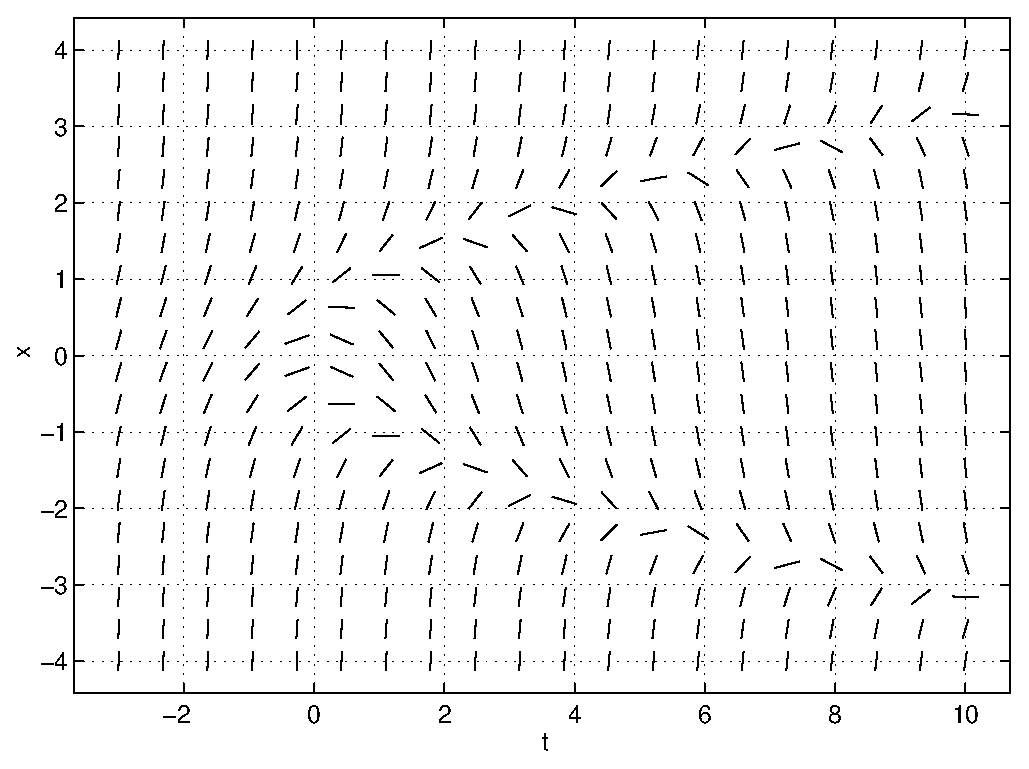
\psfig{file=../figures/df1.eps,width=3.0in}
	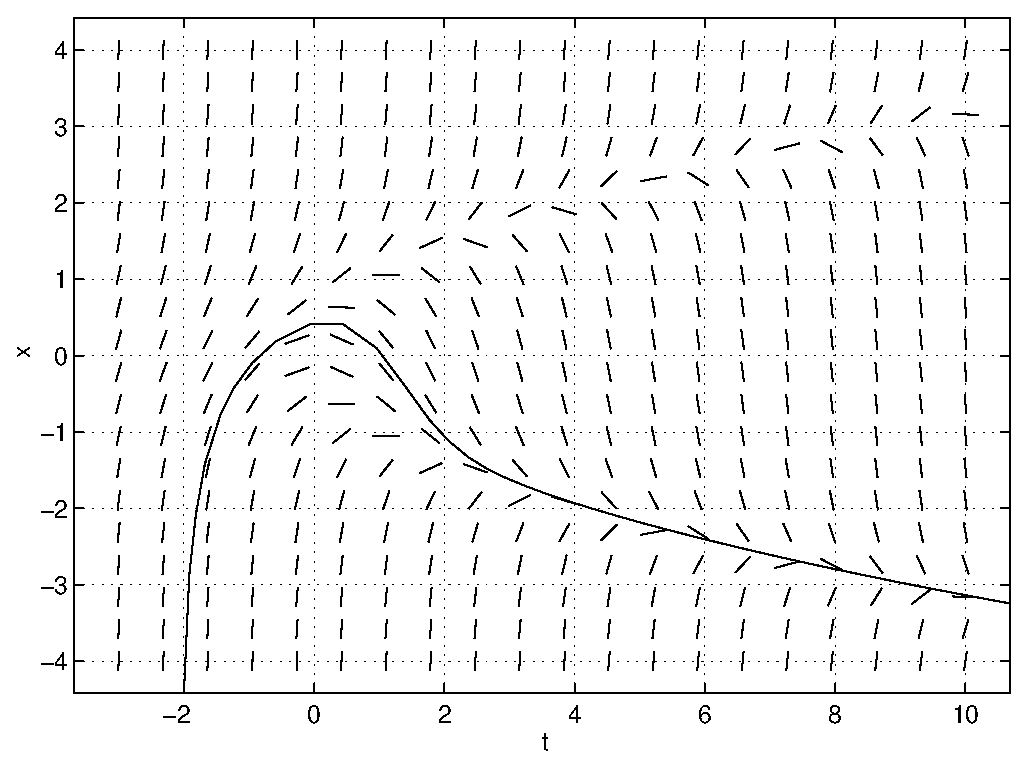
\psfig{file=../figures/df3.eps,width=3.0in}}
        \caption{Left: Line field for \protect\Ref{dfeq}
              for $t\in [-3,10]$ and $x\in [-4,4]$.
	      Right: a solution starting for $t=-2$ at $x(-2)=-4$.}
        \label{df1_labelfig}
\end{figure*}

By looking at the left hand image in Figure~\ref{df1_labelfig}
we can imagine how solution curves fit into the diagram; indeed,
we can almost use this line field to make freehand sketches
of solutions to \Ref{dfeq}.  The right hand image in
Figure~\ref{df1_labelfig} shows the solution starting at the
initial condition $x(-2) = -4$, which is the point $(x,t)=(-4,-2)$.


\subsection*{Graphing Solutions Using {\sf dfield5}}
\index{\computer!dfield5}

We now explain how to use \Matlab to display the graphs of
solutions to the differential equation \Ref{dfeq} for different
choices of initial conditions.  It is a tedious process to use
\Matlab directly to both compute and graphically display these
solutions.  Instead, we use a program written in \Matlab by John
Polking\index{Polking, John} for graphing both the line field and the time 
series of a solution to any ordinary differential equation of the form
\Ref{nonaut}.  In \Matlab this program is addressed by typing
\begin{verbatim}
dfield5
\end{verbatim}
In response, a window appears with the title {\sf
DFIELD5 Setup.}  The differential equation under consideration is 
displayed in the upper big grey frame.  In this case it is
\[
	x' = x^2 - t,
\]
which is \Ref{dfeq}.  Now use the left 
mouse button to click onto the button {\sf Proceed}.  
Then another window, having the title {\sf DFIELD5 Display},
appears.  In this window, one should see the line
field shown in Figure~\ref{df1_labelfig}.  We may compute the
solution going through the point $(t_0,x_0)=(-2,-4)$ in the
$(t,x)$-plane by clicking on that point with any mouse button.
{\sf dfield5} should reproduce the right hand side in
Figure~\ref{df1_labelfig}.

Suppose that we want to solve numerically equation \Ref{lin1}
using {\sf dfield5}. To enter this equation with $\lambda = 0.5$,
we have to change the setup.  Begin by clicking into the window
where the right hand side {\sf x\^{$\,\!$}2--t} can be found and
then replace it by {\sf 0.5*x}.  Now use the left mouse button
to click onto the button {\sf Proceed}.  In the window titled
{\sf DFIELD5 Display}, one should see the line field
\index{line field!in {\sf dfield5}} shown on
the left in Figure~\ref{df_dsp1}.
\begin{figure*}[htb]
    \centerline{%
    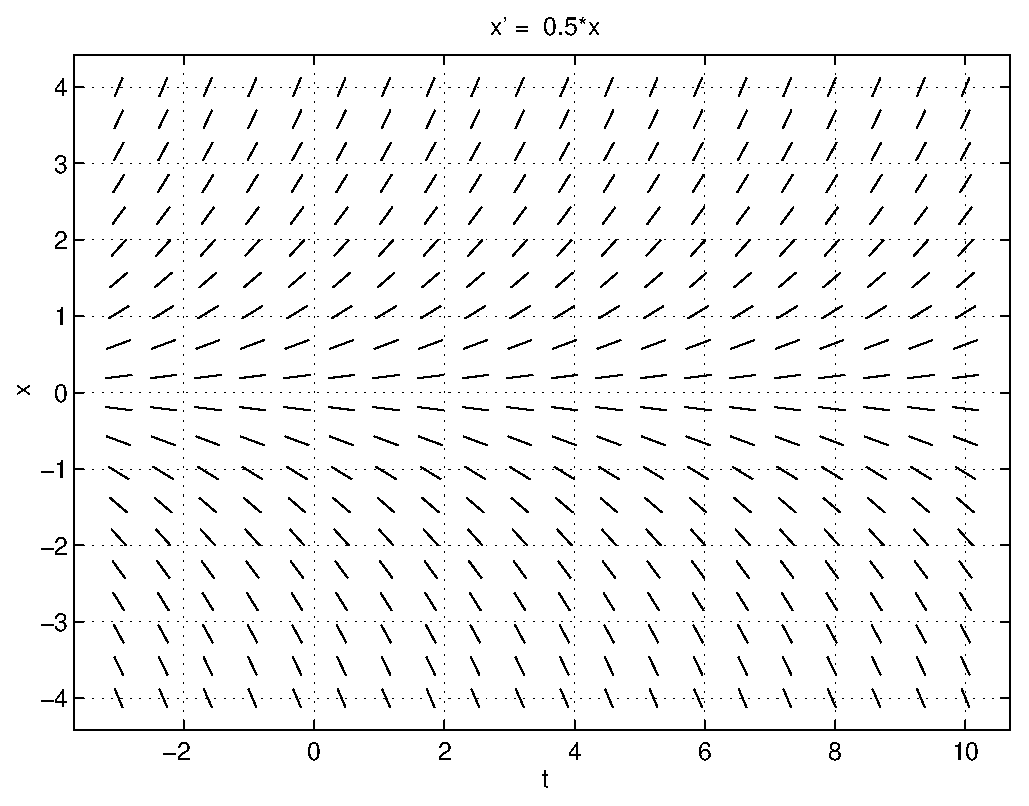
\psfig{file=../figures/df_dsp1.eps,width=3.0in}
    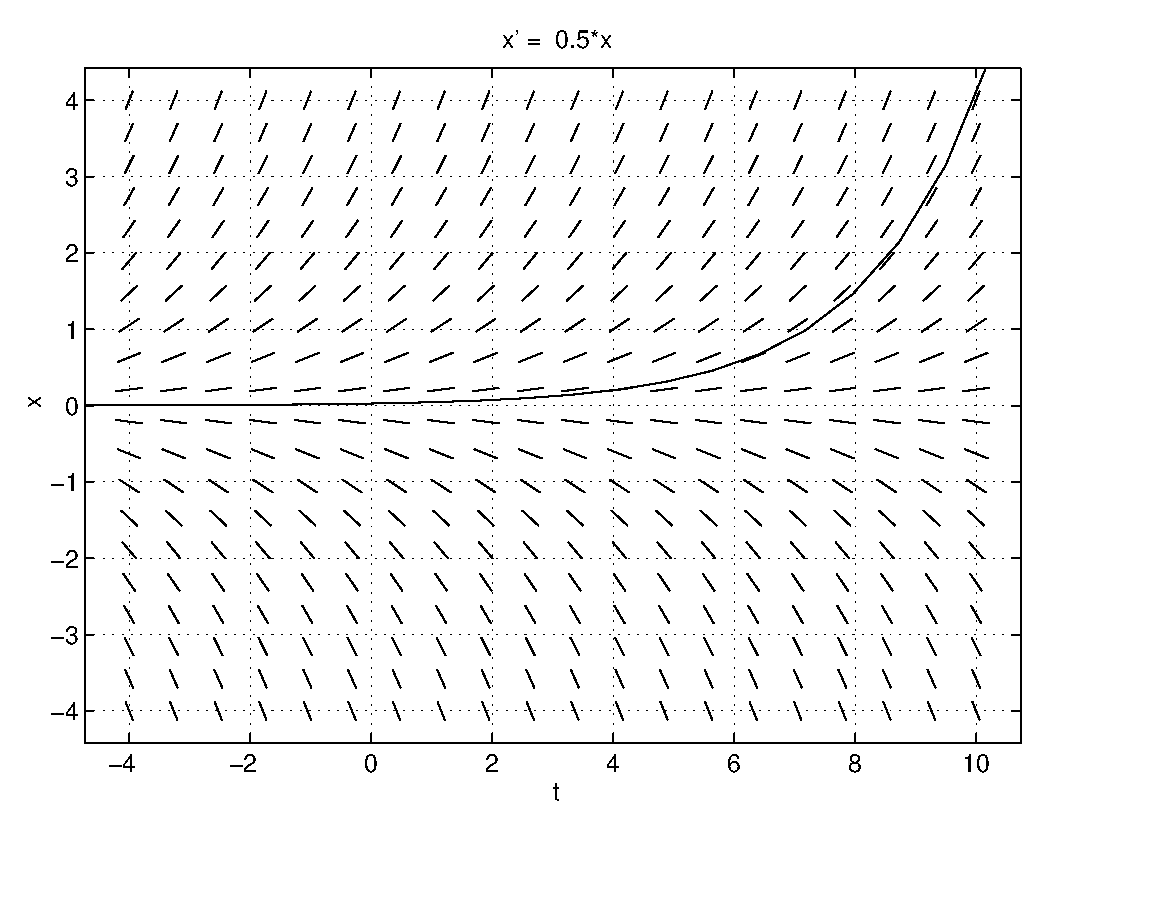
\psfig{file=../figures/dfr_dsp1.eps,width=3.0in}}
    \caption{Left: Line field for $\dot{x}=0.5x$ for $t\in [-4,10]$ and
		$x\in [-4,4]$.  Right: A solution starting at $t=0$ and
		$x>0$ but small.}
    \label{df_dsp1}
\end{figure*}

Now we may compute solutions going through a certain point
$(t_0,x_0)$ in the $(t,x)$-plane by clicking with any mouse
button on that point.  The solution is then computed first in
forward time and then in backward time.  For example, if we
click on a point near $t=x=0$ where $x>0$, {\sf dfield5} produces
the solution shown on the right in Figure~\ref{df_dsp1}.  Note
the similarity with the graph of the closed form solution in
Figure~\ref{graph_labelfig} when $\lambda=0.5$.

By clicking several times it appears that all solutions diverge
to either plus or minus infinity as $t$ goes to infinity.
Indeed, by \Ref{soln1} we know that the solutions are of the
form $x(t) = x_0 e^{0.5 t}$, and hence this behavior is expected
for $x_0\not= 0$.  To compute a solution corresponding to the case
when $x_0=0$, we bring up the menu {\sf DFIELD5 Options} and select
{\sf Keyboard input}.  This allows us to type in the initial
values $t=-2$ and $x=0$.  The action {\sf Compute} then leads to
the computation of the solution $x(t)=0$ corresponding to $x_0=0$.

The value of $\lambda=0.5$ can be changed by editing the
corresponding window in the {\sf DFIELD5 Setup.} For instance, if
we replace the $0.5$ by $-0.8$ and push {\sf Proceed}, then the
current line field is replaced by the line field shown
in Figure~\ref{df_dsp2}.
\begin{figure*}[htb]
    \centerline{%
    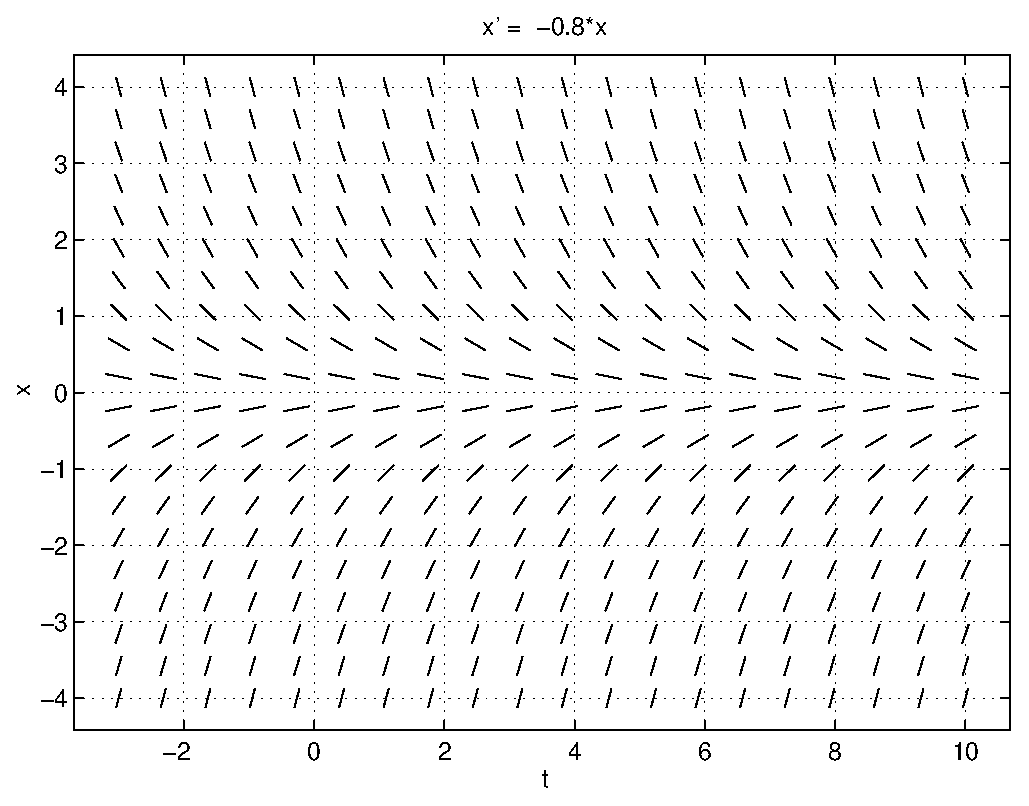
\psfig{file=../figures/df_dsp2.eps,width=3.0in}
    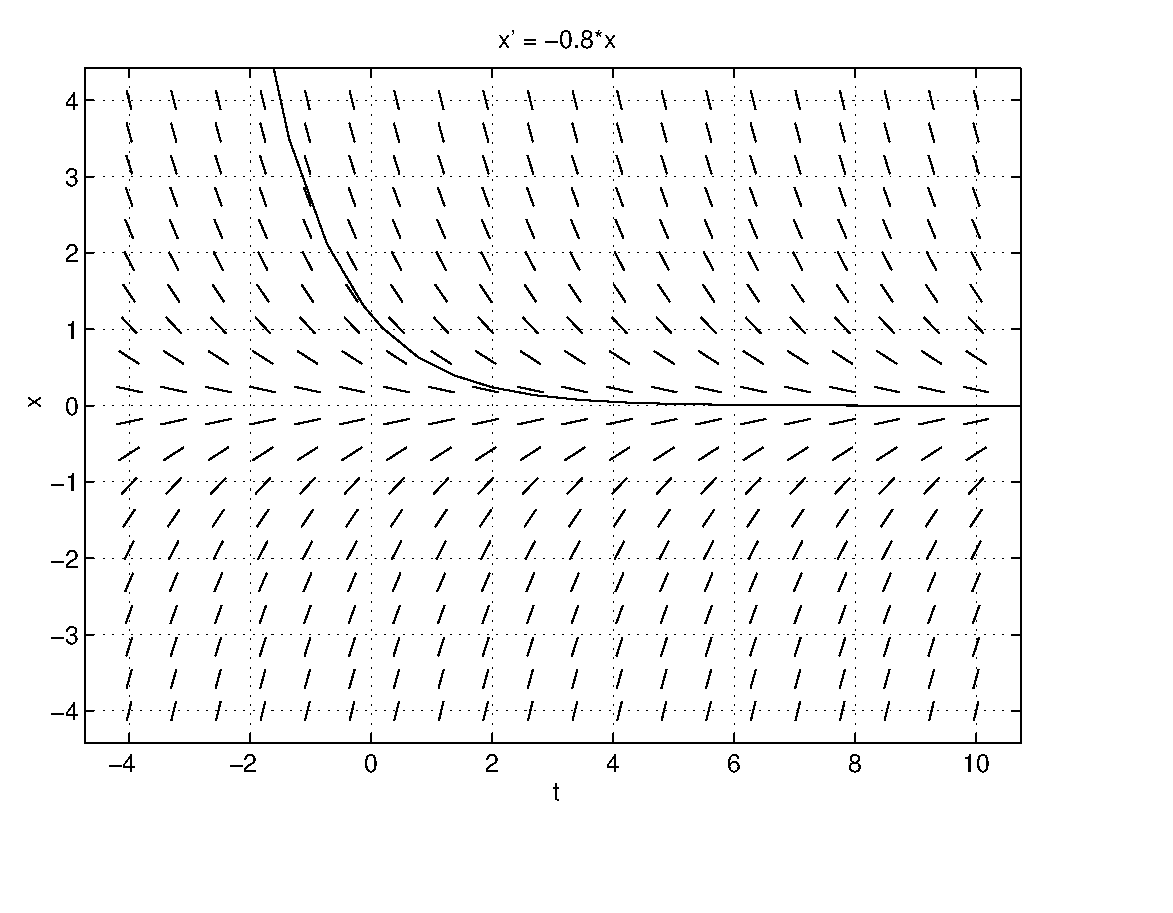
\psfig{file=../figures/dfr_dsp2.eps,width=3.0in}}
    \caption{Left: Line field for $\dot{x}=-0.8 x$ for $t\in [-4,10]$
	and $x\in [-4,4]$.  Right: A solution starting at $t=0$ and
	$x$ between $1$ and $2$.}
    \label{df_dsp2}
\end{figure*}

By computing different solutions, it seems as though all of them
converge to zero as $t$ goes to infinity, which agrees with
\Ref{explimits}.


\subsubsection*{Autonomous and Nonautonomous Equations in {\sf dfield5}}

In a sense, solutions of autonomous equations do not depend on the initial
time $t_0$, but just on the initial position $x_0$.  More precisely, let
$x_1(t)$ be the solution to
\[
\frac{dx}{dt} = f(x)
\]
with initial condition $x(0)=x_0$ and let $x_2(t)$ be a solution
to the same differential equation with initial condition $x(t_0)=x_0$.
Then
\begin{equation}  \label{E:initdiff}
x_2(t) = x_1(t-t_0).
\end{equation}
This statement can be verified by noting that the definition of
$x_2(t)$ in \Ref{E:initdiff} satisfies the initial value
\[
x_2(t_0)=x_1(t_0-t_0)=x_1(0)=x_0,
\]
and, using the chain rule, the differential equation
\[
\frac{dx_2}{dt}(t) = \frac{dx_1}{dt}(t-t_0) = f(x_1(t-t_0))=f(x_2(t)).
\]
So the solution $x_2(t)$ is the same as the solution $x_1(t)$ with
just a shift in time $t$.  In general, the same statement is {\em not\/} 
true for nonautonomous equations.

This difference between autonomous and nonautonomous equations can be
visualized using {\sf dfield5}. On the left in Figure~\ref{F:non-auto}
we graph two solutions of the {\em autonomous\/} differential equation
$\dot{x}=x^2-2x$ with initial conditions $x(0)=1$ and $x(2)=1$.  Note
that one solution is obtained from the other just by shifting by two
time units.  On the right of that figure we graph two solutions of the
{\em nonautonomous\/} differential equation $\dot{x}=x^2-t$ with
initial conditions $x(0)=1$ and $x(2)=1$.  Note that the two solutions
are most definitely not obtained one from the other by a time shift.

\begin{figure*}[htb]
        \centerline{%
        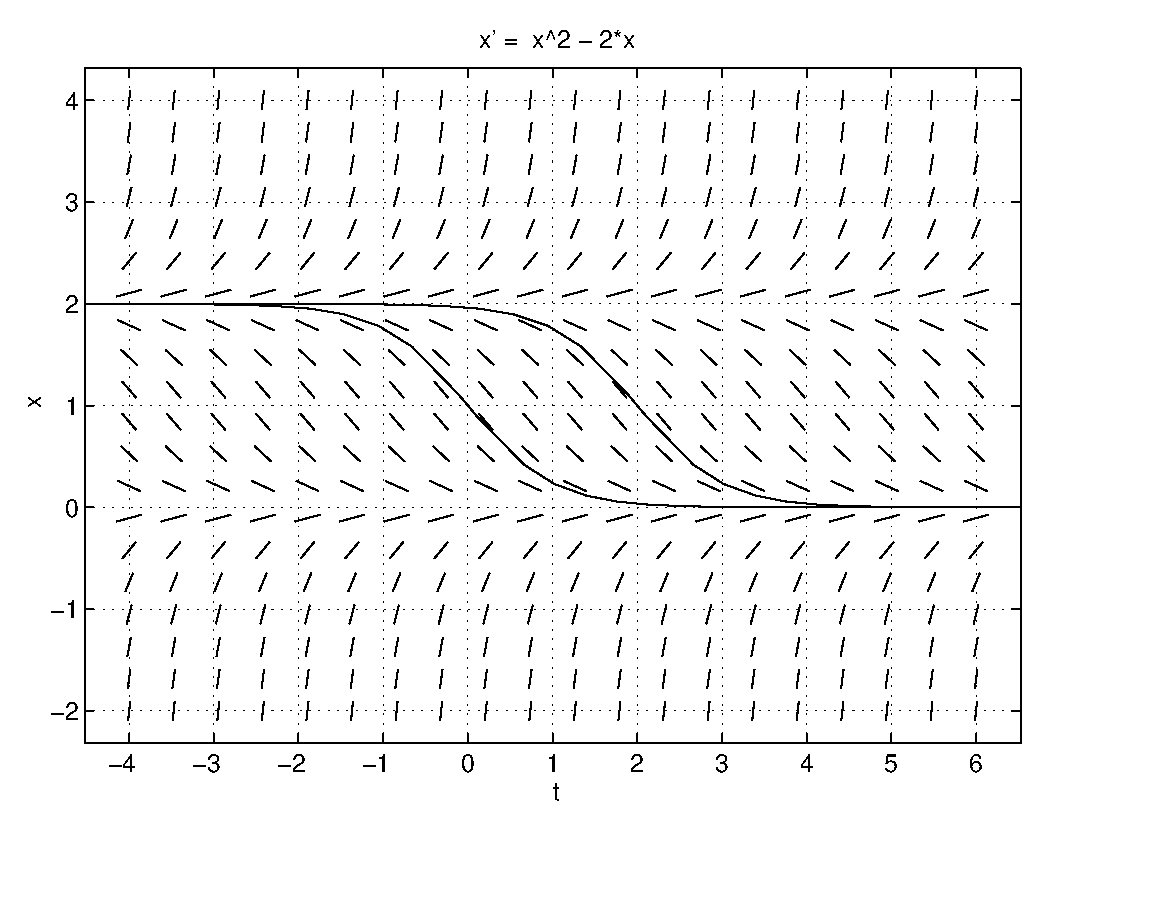
\psfig{file=../figures/auto.eps,width=3.0in}
	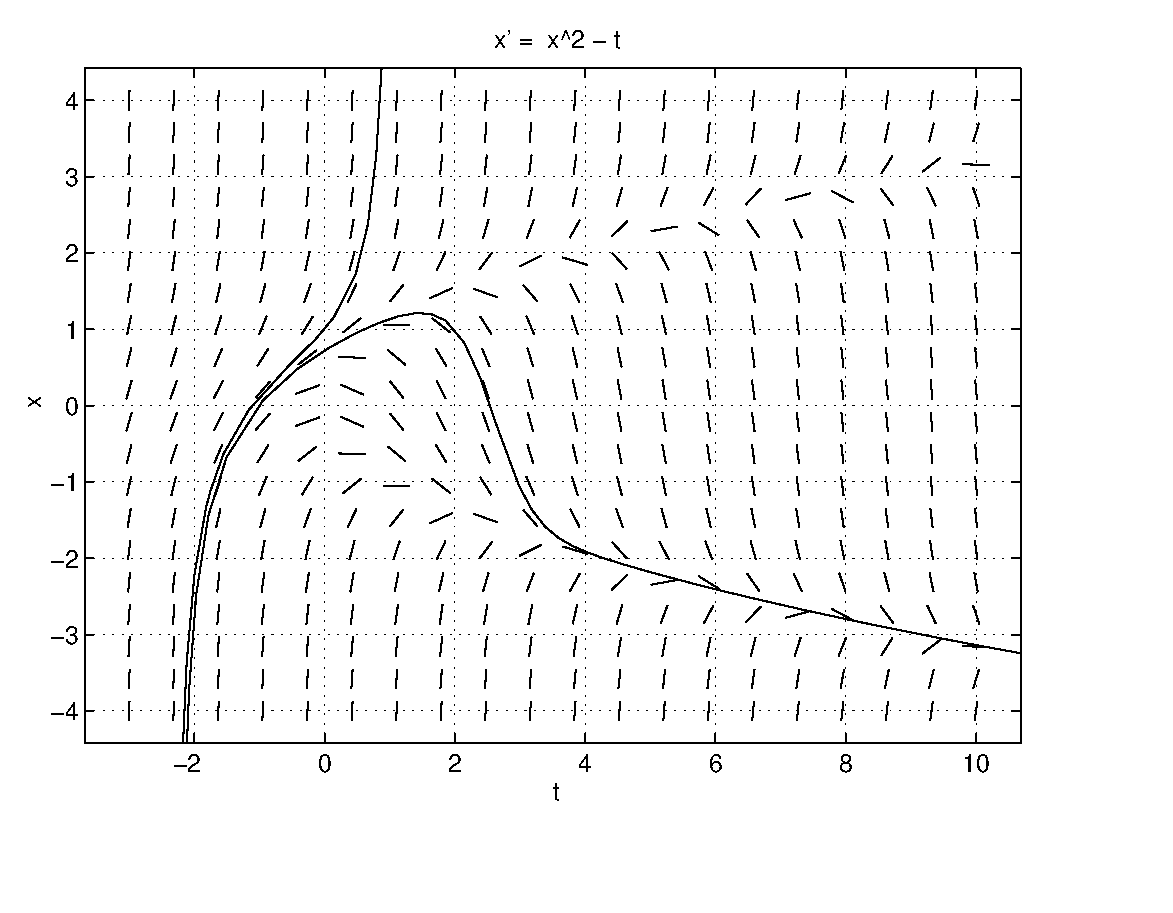
\psfig{file=../figures/nonauto.eps,width=3.0in}}
        \caption{Left: Solutions of the autonomous equation $\dot{x}=x^2-2x$
	with initial conditions $x(0)=1$ and $x(2)=1$. Right: Solution of
	the nonautonomous differential equation $\dot{x}=x^2-t$ with initial
	conditions $x(0)=1$ and $x(2)=1$.}
        \label{F:non-auto}
\end{figure*}


\EXER

\TEXER

\noindent In Exercises~\ref{c3.2.1A} -- \ref{c3.2.1D} determine whether the 
solution to the given differential equation with given initial condition is 
increasing or decreasing at the initial point.
\begin{exercise} \label{c3.2.1A}
ODE: $\dot{x}=x-t$; initial condition: $x(1)=2$.
\end{exercise}
\begin{exercise} \label{c3.2.1B}
ODE: $\dot{x}=x-t$; initial condition: $x(2)=1$.
\end{exercise}
\begin{exercise} \label{c3.2.1C}
ODE: $\dot{x}=x^2-tx$; initial condition: $x(1)=2$.
\end{exercise}
\begin{exercise} \label{c3.2.1D}
ODE: $\dot{x}=x^2-tx-t$; initial condition: $x(2)=-1$.
\end{exercise}

\noindent In Exercises~\ref{c3.2.2A} -- \ref{c3.2.2D} sketch by hand the line 
field of the given differential equation on the given rectangle.
\begin{exercise} \label{c3.2.2A}
ODE: $\dot{x}=x-t$; rectangle: $0\leq x\leq 2; -1\leq t\leq 1$.
\end{exercise}
\begin{exercise} \label{c3.2.2B}
ODE: $\dot{x}=x+t$; rectangle: $-2\leq x\leq 2; -1\leq t\leq 2$.
\end{exercise}
\begin{exercise} \label{c3.2.2C}
ODE: $\dot{x}=xt$; rectangle: $-1\leq x\leq 1; -1\leq t\leq 1$.
\end{exercise}
\begin{exercise} \label{c3.2.2D}
ODE: $\dot{x}=x/t$; rectangle: $0< x\leq 2; 0< t\leq 2$.
\end{exercise}

\noindent In Exercises~\ref{c3.2.3A} -- \ref{c3.2.3D} determine whether the 
given differential equation is autonomous or nonautonomous.
\begin{exercise} \label{c3.2.3A}
$\dot{x}=x-t$.
\end{exercise}
\begin{exercise} \label{c3.2.3B}
$\dot{x}=x^2-x$.
\end{exercise}
\begin{exercise} \label{c3.2.3C}
$\dot{x}=x\sin(x)$.
\end{exercise}
\begin{exercise} \label{c3.2.3D}
$\dot{x}=x\cos(t)$.
\end{exercise}


\CEXER

\noindent In Exercises~\ref{c3.2.a01a} -- \ref{c3.2.a01c} use
{\sf dfield5} to compute several solutions to the given differential
equations in the specified region.
\begin{exercise} \label{c3.2.a01a}
$\dot{x} = xt$, $t\in[0,2]$, $x\in[-1,1]$.
\end{exercise}
\begin{exercise} \label{c3.2.a01b}
$\dot{x} = tx^2$, $t\in[0,4]$, $x\in[-4,4]$.
\end{exercise}
\begin{exercise} \label{c3.2.a01c}
$\dot{x} = x-\sin(t)$, $t\in[-2,10]$, $x\in[-4,4]$.
\end{exercise}

\begin{exercise} \label{c3.2.1*}
Compute $x(2)$, where $x(t)$ is the solution to the differential equation 
$\dot{x} = 0.6x$ with initial condition $x(0)=0.5$, in two different ways, 
as follows:
\begin{itemize}
\item[(a)] Use {\sf Keyboard input} in {\sf dfield5} to compute the 
solution with initial value $x(0)=0.5$.  Use the {\sf zoom in} feature in 
the {\sf DFIELD5 Edit} menu to compute $x(2)$ to an accuracy of two decimal 
places.  (Drag a rectangle around the point you are interested in.  Repeat 
this several times until you can read off the value $x(2)$ of the solution.)  
\item[(b)] Use \Matlab to compute the value of the exact solution
of the form \Ref{soln1} with initial value $x(0)=0.5$.  
\item[(c)] Is your answer obtained using {\sf dfield5} in (a) accurate to 
within two decimal places of the answer obtained using (b)?  If not, 
which answer do you trust more, and why?
\end{itemize}
\end{exercise}

\begin{exercise} \label{c3.2.2}
Use {\sf dfield5} to compute solutions to the differential equation
$\dot{x} = x^2-tx+2t$. Use {\sf Keyboard input} to compute the solution
with initial value $x(-1)=-1$.  What is the minimum value of this
solution $x(t)$ on the interval $-2\leq t\leq 1$?  Plot
solutions to this equation starting with at least six or seven
different initial conditions. Then print the result.
\end{exercise}

\begin{exercise} \label{c3.2.3}
Use {\sf dfield5} to compute solutions to the differential
equation
\begin{equation}  \label{E:freehand}
\dot{x} = x^3-2t^2x-t.
\end{equation}
Print the line field of \Ref{E:freehand} on the intervals
$t\in[-2,2]$ and $x\in[-2,3]$.  Use the line field to draw freehand
the solution to \Ref{E:freehand} starting at $(t_0,x_0)=(-2,1)$.
Then set the initial condition using {\sf Keyboard input}
and print the numerically computed solution. Finally, compare
your freehand drawing with the numerically computed result.
\end{exercise}

\begin{exercise}  \label{exer:at}
\begin{itemize}
\item[(a)]  Draw the direction field for
\begin{equation} \label{ex:at}
\frac{dx}{dt} = \frac{x}{x-t}.
\end{equation}
Assuming that $x(2)=3$, estimate $x(137)$.
\item[(b)]  Verify that
\[
x(t) = t + \sqrt{t^2-3}
\]
is the solution to \Ref{ex:at}.  Then show that $x(t)$ satisfies the
initial condition $x(2)=3$.
\item[(c)]  Compare your estimate of the solution to \Ref{ex:at}
obtained using {\sf dfield5} with the exact solution
\[
x(137)= 137 +\sqrt{18766} \approx 273.989
\]
\end{itemize}
\end{exercise}

\end{document}
